% --------- TEMPLATE FOR A THESIS IN ECONOMICS -------------- %
%   Made by Hugo Norinder
%   First created: 2024-05-22
%   Updated: 2024-05-22
%
%
%This template was made to guide students in making a thesis that looks like a publishable article
% ---------- ********************************* -------------- %

\documentclass[a4paper, 12pt]{article}
%------ SETUP OF THE DOCUMENT ------%
%This part of the document sets up the document and makes it easier to read the main.tex file
%Changes in the setup file are recommended if you wish to customize things like colors in links and such.

%------ ********************* ------%
\usepackage[margin = 25mm]{geometry} %
\usepackage{graphicx} % Required for inserting images
\usepackage[toc,page]{appendix}
\usepackage[english=usenglishmax]{hyphsubst} %sets hyphenation to American English. Google is your friend on hyphenation. Babel could also be used
\usepackage[hyphens]{url}
\usepackage{amsmath, amssymb, setspace, float, subcaption, caption, booktabs, pdflscape, dcolumn, titlesec, tocloft, comment, xcolor, longtable, blindtext, rotating, lipsum}
\usepackage[flushleft]{threeparttable}
\usepackage[round, numbers, authoryear]{natbib}
\usepackage[hidelinks]{hyperref}
\usepackage{titlesec}
\usepackage{enumitem}

\hypersetup{
     colorlinks   = true, %If links to papers should be colored
     citecolor    = blue, %color of citation text
     urlcolor = blue, %if you use an URL, this is how it is colored
    linkcolor = black
}

\graphicspath{{figures/}}

%CHANGE SECTION STYLE

\bibliographystyle{apalike} %closest to LUSEM Harvard referencing guide

%%%%%%%%%%%%%%%%%%%%%%%%%%%%%%%%%%%
% Table formatting
%%%%%%%%%%%%%%%%%%%%%%%%%%%%%%%%%%%
\usepackage{multirow}


%%%%%%%%%%%%%%%%%%%%%%%%%%%%%%%%%%%
% Equation Formatting
%%%%%%%%%%%%%%%%%%%%%%%%%%%%%%%%%%%
\numberwithin{equation}{section}

%%%%%%%%%%%%%%%%%%%%%%%%%%%%%%%%%%%
% List Formatting
%%%%%%%%%%%%%%%%%%%%%%%%%%%%%%%%%%%
\setlist[itemize]{itemsep=0.05em}

\title{Means Testing in BAföG: The Impact of Income Eligibility Thresholds on Student Labor Supply
\footnote{\textbf{Acknowledgement:} You can thank who you want, but it is common to thank you supervisor(s), commenters, or other people you think deserve a mention
}}
\author{
María Sól Antonsdóttir 
\and 
Alexander Eriksson Byström
}
\date{Seminar date}
\begin{document}

%THE UNFORTUNATE TITLE PAGE THAT NEEDS TO BE INCLUDED
\setstretch{1.5}

    %
\includegraphics[scale = 0.3]{images/LU RGB.png}
    %
\includegraphics[scale = 0.3]{images/LU Black.png} 
    
\includegraphics[scale = 0.15]{images/LUSEM_RGB.png} %I recommend using this one but the others are fine too
    %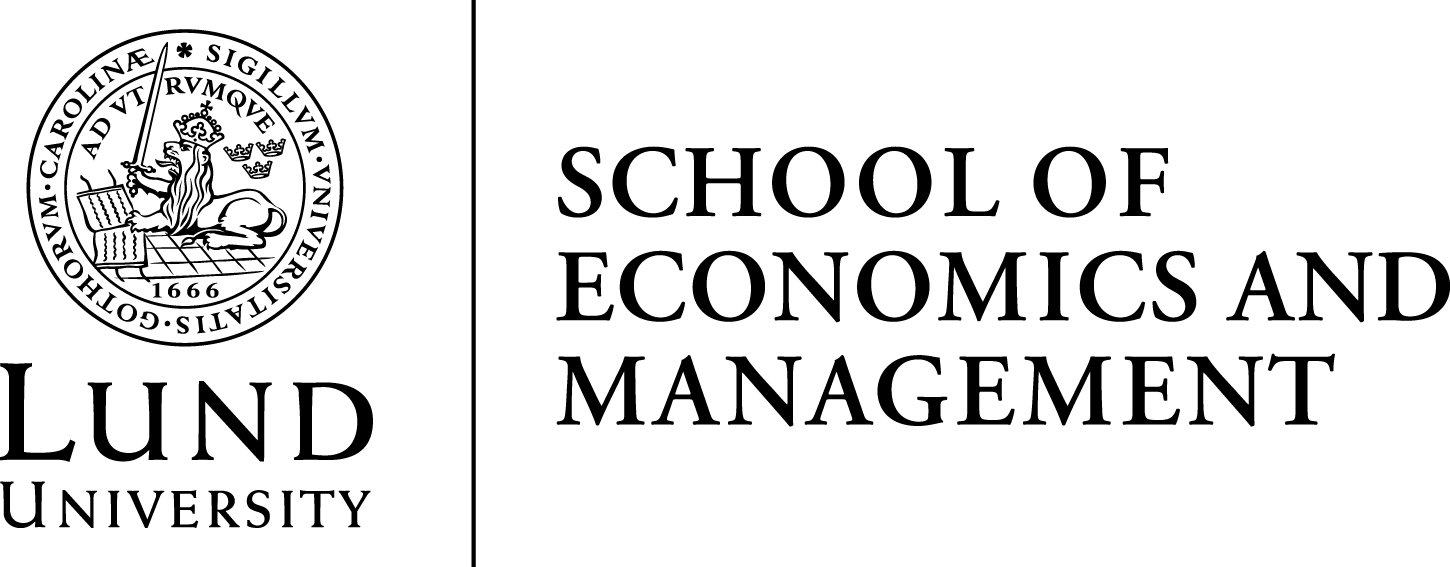
\includegraphics[scale = 0.15]{images/LUSEM_BLACK.png}

\vspace{2cm}
    \begin{center}       
        \vspace*{2cm}
        {\LARGE {\textbf{Means Testing in BAföG}  \\
        The Impact of Income Eligibility Thresholds on Student Labor Supply
        }} \\
        \vspace{1cm}
        \Large{María Sól Antonsdóttir \& Alexander Eriksson Byström} \normalsize{\\ Department of Economics \\ Lund University School of Economics and Management}
    \end{center}
    \vspace{2cm}

\vfill
\noindent 
\textbf{Supervisor: Petra Thiemann} \\ 
NEKN01 - Master Thesis in Economics 15 ECTS \\ 
Seminar date: Month Day, Year
\thispagestyle{empty}

\newpage
\tableofcontents
\thispagestyle{empty}

\newpage
%\maketitle
\begin{abstract}
\setstretch{1}
\lipsum[1] \\
    \noindent \textbf{Keywords:}  3 -- 5 key words\\
    \noindent \textbf{JEL codes:} Find appropriate codes at
    \url{https://www.aeaweb.org/econlit/jelCodes.php?view=jel}  %Standard in econ literature view=jel
\end{abstract}
\newpage
\setcounter{page}{1}

%INTRODUCTION
\hypersetup{linkcolor=blue}
\section{Introduction} \label{sec:intro}
test \cite{xkcd}


%PREVIOUS LITERATURE
\section{LITERATURE} \label{sec:literature}


%REFERENCES
\titleformat{\section}{\normalfont\huge\bfseries}{\thesection}{1em}{} 
\newpage
\addcontentsline{toc}{section}{References} 
\bibliography{bibliography}
\newpage

%APPENDICES
\appendix
\setcounter{page}{1} %Restarts page counting to 1
\pagenumbering{roman} %Differentiates the appendix page numbers from the main article

\titleformat{\section}{\centering\normalfont\normalsize\bfseries}{Appendix \thesection: }{0em}{}
\newpage
\section{Tables}
\renewcommand{\thetable}{\thesection \arabic{table}}
\setcounter{table}{0}


\begin{table}[H]
\centering
\renewcommand{\arraystretch}{0.8}  % Increase the height of the header
\begin{tabular}{lrrrr}
\hline
\hline
Year & \multicolumn{3}{c}{(\%) Supported Students} & Avg. Monthly Payment (2023 prices) \\
\cline{2-4}
     & Partially & Fully & Total & \\
\hline
1998 & 13 & 5 & 19 & 498.34 \\
1999 & 13 & 6 & 19 & 502.83 \\
2000 & 14 & 6 & 19 & 503.90 \\
2001 & 15 & 7 & 22 & 553.19 \\
2002 & 15 & 9 & 23 & 554.36 \\
2003 & 15 & 9 & 24 & 547.26 \\
2004 & 16 & 10 & 25 & 539.85 \\
2005 & 16 & 10 & 26 & 536.96 \\
2006 & 16 & 10 & 25 & 528.53 \\
2007 & 16 & 10 & 25 & 516.68 \\
2008 & 14 & 11 & 25 & 534.48 \\
2009 & 16 & 10 & 26 & 580.82 \\
2010 & 16 & 10 & 27 & 577.54 \\
2011 & 17 & 10 & 27 & 586.09 \\
2012 & 17 & 10 & 27 & 570.14 \\
2013 & 16 & 10 & 25 & 559.06 \\
2014 & 15 & 9 & 24 & 556.19 \\
2015 & 14 & 8 & 22 & 553.24 \\
2016 & 12 & 8 & 21 & 569.99 \\
2017 & 12 & 8 & 20 & 604.08 \\
2018 & 10 & 8 & 18 & 586.47 \\
2019 & 10 & 7 & 17 & 602.85 \\
2020 & 9 & 7 & 16 & 669.86 \\
2021 & 9 & 7 & 16 & 655.38 \\
2022 & 8 & 8 & 17 & 647.04 \\
2023 & 9 & 9 & 17 & 663.00 \\
\hline
\end{tabular}
\caption{
  Descriptives from 1998--2023 showing the fraction of HE students partially and fully 
  supported by BAföG, along with the average monthly payment adjusted for the German Consumer Price Index (CPI) from Destatis.
}
\label{tab:support_fraction_financial_expenditure}
\end{table}

\newpage
\section{Figures}
\renewcommand{\thefigure}{\thesection \arabic{figure}}
\setcounter{figure}{0}

\begin{figure}[H]
  \centering
  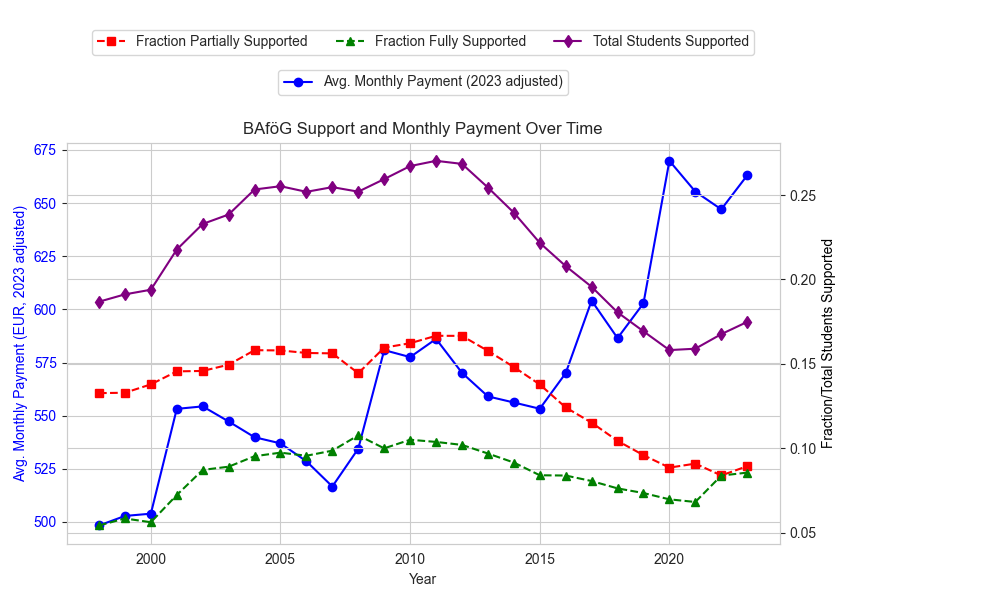
\includegraphics[width=0.95\linewidth]{bafog_support_over_time.png}
  \caption{
      Trends in CPI-adjusted average monthly payments from 1998 to 2023, expressed in 2023 prices. The figure also illustrates the fraction of enrolled students in Germany receiving partial, full, or combined partial and full loans and grants over the same period.
  }
  \label{fig:test}
\end{figure}

\end{document}
